\documentclass[aspectratio=169,10pt]{beamer}
\usetheme{Madrid}
\usecolortheme{seahorse}

\usepackage{amsmath}
\usepackage{amssymb}
\usepackage{amsfonts}
\usepackage{mathtools}
\usepackage{listings}
\usepackage{xcolor}
\usepackage{array}
\usepackage{booktabs}
\usepackage{tikz}

\graphicspath{{figures/}}

% Set footline
\setbeamertemplate{footline}[frame number]

% Code formatting
\lstset{
    basicstyle=\ttfamily\scriptsize,
    numbers=left,
    numberstyle=\tiny\color{gray},
    frame=single,
    breaklines=true,
    commentstyle=\color{green!50!black}\itshape,
    keywordstyle=\color{blue}\bfseries,
    stringstyle=\color{red},
    showstringspaces=false,
    language=Python
}

\title{Chapter 24: Proximity Operators}
\subtitle{Convex Analysis and Monotone Operator Theory}
\author{Based on Bauschke \& Combettes (2017)}
\date{}

\begin{document}

%===============================================================================
\begin{frame}
\titlepage
\end{frame}

%===============================================================================
\begin{frame}[allowframebreaks]{Overview}
\tableofcontents
\end{frame}

%===============================================================================
\section{Introduction to Proximity Operators}
%===============================================================================

\begin{frame}{What is a Proximity Operator?}
\begin{block}{Definition}
For a function $f \in \Gamma_0(\mathcal{H})$ and $\gamma \in \mathbb{R}_{++}$, the \textbf{proximity operator} is:
\[
\mathrm{Prox}_{\gamma f}(x) := \argmin_{p \in \mathcal{H}} \left( f(p) + \frac{1}{2\gamma}\|p - x\|^2 \right)
\]
\end{block}

\vspace{0.3cm}

\begin{itemize}
    \item $f$: proper, convex, lower-semicontinuous function
    \item $\gamma > 0$: step size or regularization parameter
    \item The argmin is \textbf{unique} (strong convexity)
\end{itemize}

\vspace{0.3cm}

\begin{exampleblock}{Interpretation}
Balances two goals:
\begin{enumerate}
    \item Minimize $f(p)$
    \item Stay close to the original point $x$
\end{enumerate}
\end{exampleblock}
\end{frame}

\begin{frame}{Basic Characterization}
\begin{theorem}[Characterization via Subdifferential]
For $f \in \Gamma_0(\mathcal{H})$, $x \in \mathcal{H}$, and $\gamma \in \mathbb{R}_{++}$:
\[
p = \mathrm{Prox}_{\gamma f}(x) \iff 0 \in \partial f(p) + \frac{1}{\gamma}(p - x)
\]
\end{theorem}

\vspace{0.3cm}

\begin{corollary}
Equivalently:
\[
p = \mathrm{Prox}_{\gamma f}(x) \iff x - p \in \gamma \partial f(p)
\]
\end{corollary}

\vspace{0.3cm}

\begin{example}
If $f$ is differentiable at $p$:
\[
x - p = \gamma \nabla f(p) \implies p = x - \gamma \nabla f(p)
\]
This is a \textbf{gradient descent step}!
\end{example}
\end{frame}

\begin{frame}{Proximity Operators as Resolvents}
\begin{theorem}[Connection to Monotone Operators]
For $A = \partial f$ (maximally monotone by Theorem 20.25):
\[
\mathrm{Prox}_{\gamma f} = (\mathrm{Id} + \gamma A)^{-1}
\]
\end{theorem}

\vspace{0.3cm}

\begin{itemize}
    \item $\mathrm{Prox}_{\gamma f}$ is the \textbf{resolvent} of the monotone operator $\partial f$
    \item Key property: For all $f \in \Gamma_0(\mathcal{H})$:
    \[
    J_{\gamma \partial f} = \mathrm{Prox}_{\gamma f}
    \]
    \item Single-valued and nonexpansive operator
\end{itemize}

\vspace{0.4cm}

\begin{corollary}[Relationship to Zeros]
Finding $p$ such that $0 \in \partial f(p)$ is equivalent to finding fixed points of $\mathrm{Prox}_{\gamma f}$.
\end{corollary}
\end{frame}

\begin{frame}{Proximity Operators and Gradients}
\begin{theorem}[Characterization via Gradients]
Let $T: \mathcal{H} \to \mathcal{H}$, $f \in \Gamma_0(\mathcal{H})$, and $q = \frac{1}{2}\|\cdot\|^2$. Then:
\begin{enumerate}
    \item $T = \mathrm{Prox}_f$
    \item $T = \nabla(f + q)^*$
    \item $T = \nabla(f^* \square q) = \nabla({}^!(f^*))$
\end{enumerate}
are equivalent.
\end{theorem}

\vspace{0.3cm}

\begin{corollary}
For $f, g \in \Gamma_0(\mathcal{H})$ with $f = g - \frac{1}{2}\|\cdot\|^2$:
\[
\mathrm{Prox}_f = \nabla g^*
\]
\end{corollary}
\end{frame}

%===============================================================================
\section{Basic Properties of Proximity Operators}
%===============================================================================

\begin{frame}[allowframebreaks]{Key Properties}
\begin{property}[Composition Rules]
Let $f, g \in \Gamma_0(\mathcal{H})$. We have:
\begin{enumerate}
    \item If $g = f + \frac{\alpha}{2}\|\cdot - z\|^2 + \langle u \rangle + \beta$:
    \[
    \mathrm{Prox}_g x = \mathrm{Prox}_{(1+\alpha)^{-1}f}\left((1+\alpha)^{-1}(x + \alpha z - u)\right)
    \]
    \item If $g = z + \mathrm{Prox}_{tf}(x - z)$ where $L$ is invertible:
    \[
    \mathrm{Prox}_g x = L^*(\mathrm{Prox}_{f \circ L}(Lx))
    \]
    \item If $\mathrm{Prox}_f = \mathrm{Prox}_g$: There exists $\gamma \in \mathbb{R}$ such that $f = g + \gamma$.
\end{enumerate}
\end{property}

\framebreak

\begin{property}[Scaling and Operations]
\begin{enumerate}
    \item Scaling: $\mathrm{Prox}_{\mu f} x = x + \frac{\gamma}{\mu}(\mathrm{Prox}_{\gamma\mu f} x - x)$
    \item Reflection: If $f$ is even, then $\mathrm{Prox}_f$ is odd and $\mathrm{Prox}_f 0 = 0$
    \item Conjugate: For $f^*$, $\mathrm{Prox}_{f^*} x = x - \gamma \mathrm{Prox}_{\gamma^{-1}f}(\gamma^{-1}x)$
\end{enumerate}
\end{property}
\end{frame}

\begin{frame}{Weak Sequential Continuity}
\begin{theorem}[Weak Sequential Continuity]
For $f \in \Gamma_0(\mathcal{H})$:
\begin{enumerate}
    \item $\mathrm{Prox}_f$ is weakly sequentially continuous
    \item If $(x_n)_{n \in \mathbb{N}}$ is a sequence with $x_n \rightharpoonup x$, then:
    \[
    \|\mathrm{Prox}_f x_n\| \leq \|x_n\|
    \]
    \item Therefore $(\mathrm{Prox}_f x_n)_{n \in \mathbb{N}}$ is bounded, and $\mathrm{Prox}_f x_n \rightharpoonup \mathrm{Prox}_f x$
\end{enumerate}
\end{theorem}

\vspace{0.3cm}

\begin{corollary}
Proximity operators are \textbf{continuous} (strong topology) and have strong convergence properties.
\end{corollary}
\end{frame}

\begin{frame}{Composition of Proximity Operators}
\begin{theorem}[Composition Rule]
Let $f, g \in \Gamma_0(\mathcal{H})$. If one of the following holds:
\begin{enumerate}
    \item $(\forall y \in \mathrm{dom} \partial g)\ \partial g(y) \subseteq \partial(\mathrm{Prox}_f y)$
    \item $(\forall (x,u) \in \mathrm{gra} \partial f)\ \partial g(x + u) \subseteq \partial(x)$
    \item $\mathrm{dom} g$ is open, $g$ is Gâteaux differentiable on $\mathrm{dom} g$, $\mathrm{dom} \partial f \subset \mathrm{dom} g$, and $(\forall y \in \mathrm{dom} g)\ \nabla g(y) = \nabla g(\mathrm{Prox}_f y)$
    \item $0 \in \mathrm{sri}(\mathrm{dom} f - \mathrm{dom} g)$ and $(\forall (x,u) \in \mathrm{gra} \partial f)\ \partial g(x) \subseteq \partial(x + u)$
\end{enumerate}
Then:
\[
\mathrm{Prox}_{f+g} = \mathrm{Prox}_f \circ \mathrm{Prox}_g
\]
\end{theorem}
\end{frame}

%===============================================================================
\section{Examples of Proximity Operators}
%===============================================================================

\begin{frame}{Example 1: Quadratic Functions}
\begin{example}[Self-Adjoint and Monotone Operator]
Let $L \in \mathcal{B}(\mathcal{H})$ be self-adjoint and monotone, $u \in \mathcal{H}$, $\alpha \in \mathbb{R}$. Set:
\[
f: \mathcal{H} \to \mathbb{R}, \quad x \mapsto \frac{1}{2}\langle Lx \,|\, x \rangle + \langle u \,|\, x \rangle + \alpha
\]
Then $f \in \Gamma_0(\mathcal{H})$ and:
\[
(\forall x \in \mathcal{H})\ \mathrm{Prox}_f x = \left(\mathrm{Id} + L\right)^{-1}(x - u)
\]
\end{example}

\vspace{0.3cm}

\begin{example}[Weighted Norm Squared]
Let $I$ be a finite index set, $(\mathcal{K}_i)_i$, $(r_i)_i$, $(\lambda_i)_i$ given. Set:
\[
f(x) = \frac{1}{2}\sum_{i \in I} \lambda_i \|L_i^* x - r_i\|^2
\]
Then:
\[
(\forall x \in \mathcal{H})\ \mathrm{Prox}_f x = \left(\mathrm{Id} + \sum_{i \in I} \lambda_i L_i^* L_i\right)^{-1}\left(x + \sum_{i \in I} \lambda_i L_i^* r_i\right)
\]
\end{example}
\end{frame}

\begin{frame}{Example 2: Soft Thresholding}
\begin{example}[Soft Thresholding for $\ell_1$ Norm]
For $\gamma \in \mathbb{R}_{++}$ and $x \in \mathcal{H}$:
\[
\mathrm{Prox}_{\gamma \|\cdot\|_1} x = \begin{cases}
\left(1 - \frac{\gamma}{\|x\|}\right)x & \text{if } \|x\| > \gamma \\
0 & \text{if } \|x\| \leq \gamma
\end{cases}
\]
\end{example}

\vspace{0.3cm}

This is also called \textbf{soft thresholding} or \textbf{shrinkage} operator.

\vspace{0.3cm}

\begin{center}
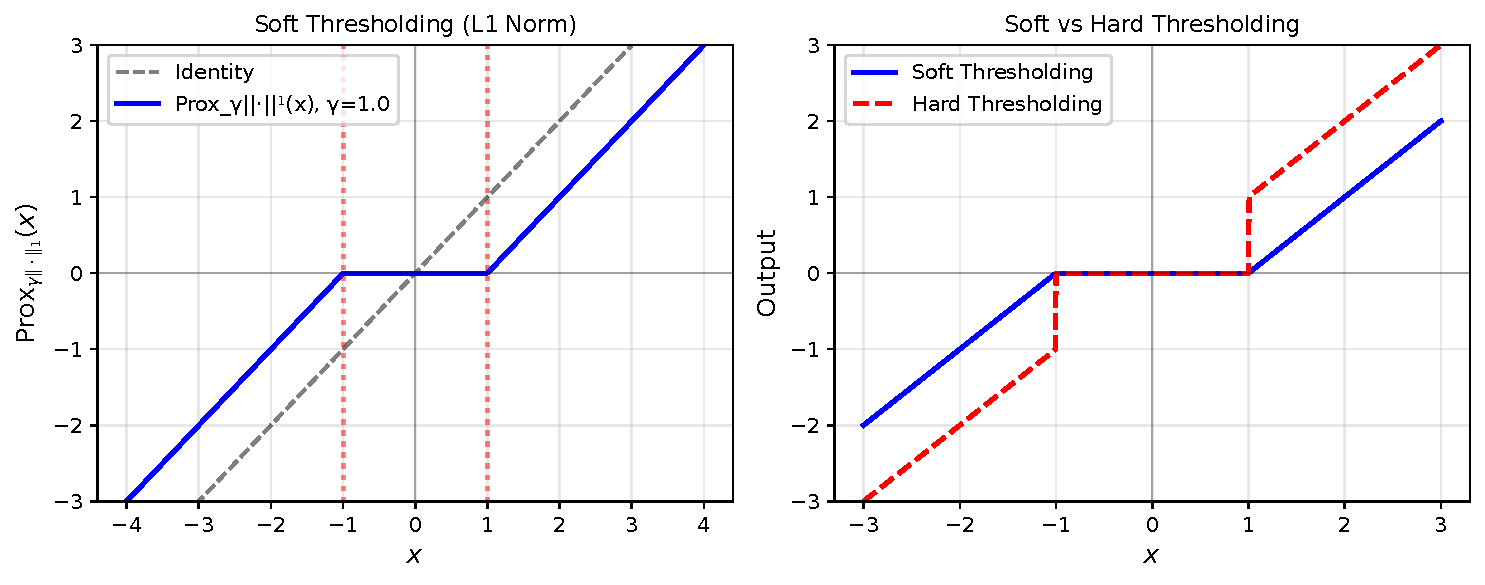
\includegraphics[width=0.6\textwidth]{fig_soft_thresholding.pdf}
\end{center}
\end{frame}

\begin{frame}{Example 3: Huber Function}
\begin{example}[Generalized Huber Function]
The function:
\[
f: \mathcal{H} \to \mathbb{R}, \quad x \mapsto \begin{cases}
\rho\|x\| - \frac{\rho^2}{2} & \text{if } \|x\| > \rho \\
\frac{\|x\|^2}{2} & \text{if } \|x\| \leq \rho
\end{cases}
\]
with $\gamma \in \mathbb{R}_{++}$ gives:
\[
(\forall x \in \mathcal{H})\ \mathrm{Prox}_{\gamma f} x = \begin{cases}
\left(1 - \frac{\gamma\rho}{\|x\|}\right)x & \text{if } \|x\| > (\gamma + 1)\rho \\
\frac{1}{\gamma + 1}x & \text{if } \|x\| \leq (\gamma + 1)\rho
\end{cases}
\]
\end{example}

\begin{center}
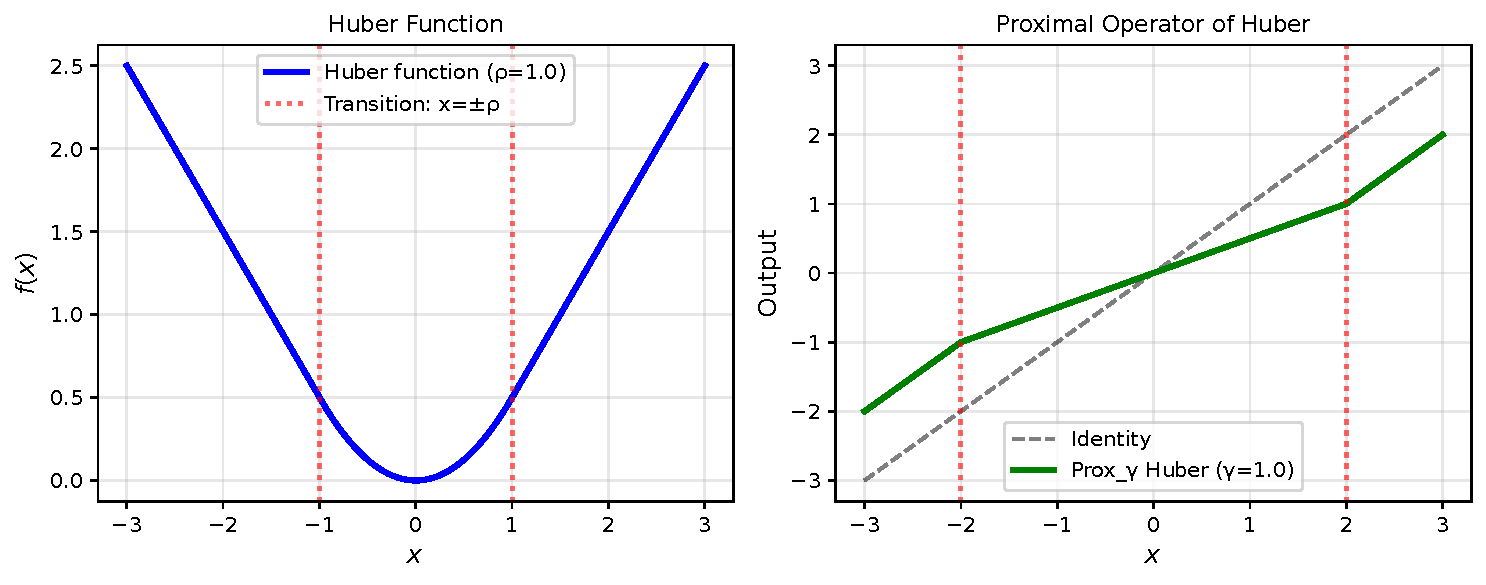
\includegraphics[width=0.5\textwidth]{fig_huber_function.pdf}
\end{center}
\end{frame}

\begin{frame}{Example 4: Indicator Functions}
\begin{example}[Projection onto Convex Set]
Let $C$ be a nonempty closed convex subset of $\mathcal{H}$. The indicator function $\iota_C$ satisfies:
\[
\mathrm{Prox}_{\iota_C} = P_C
\]
i.e., the proximity operator is the \textbf{projection} onto $C$.
\end{example}

\vspace{0.3cm}

\begin{center}
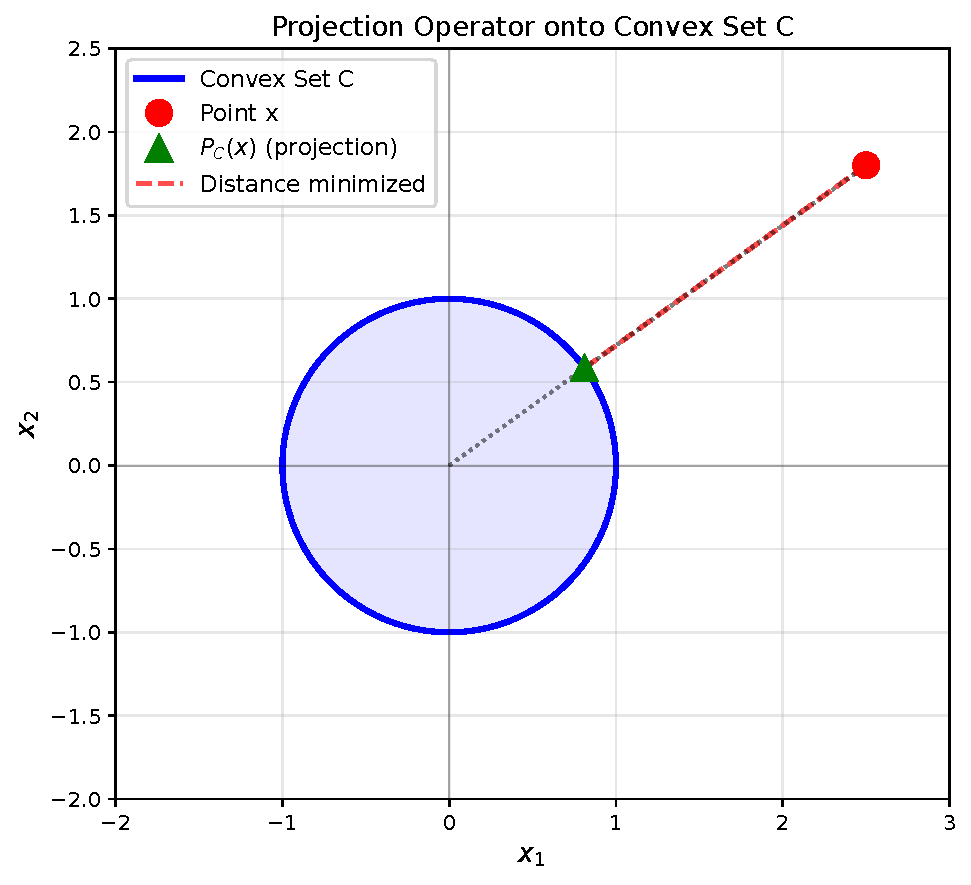
\includegraphics[width=0.5\textwidth]{fig_projection_operator.pdf}
\end{center}

\vspace{0.2cm}

Key insight: \textbf{Projections are special cases of proximity operators!}
\end{frame}

%===============================================================================
\section{Distance-Based Functions}
%===============================================================================

\begin{frame}{Distance Functions in Optimization}
\begin{definition}[Distance Function]
For a nonempty closed convex set $C \subseteq \mathcal{H}$:
\[
d_C(x) := \inf_{p \in C} \|x - p\|
\]
\end{definition}

\vspace{0.3cm}

\begin{theorem}[Subdifferential of Distance Function]
For $x \notin C$:
\[
\partial d_C(x) = \begin{cases}
\{(P_C x - x)/\|x - P_C x\|\} & \text{if } d_C(x) > \max \mathrm{Argmin} \phi; \\
P_C x & \text{if } d_C(x) \leq \max \mathrm{Argmin} \phi
\end{cases}
\]
\end{theorem}

\vspace{0.3cm}

\begin{corollary}
The proximity operator of $f = \phi \circ d_C$ depends on whether the distance to $C$ exceeds a threshold.
\end{corollary}
\end{frame}

\begin{frame}{Proximal Operators of Distance Compositions}
\begin{proposition}[Distance-Based Composition]
Let $C$ be a nonempty closed convex set, $\phi: \mathbb{R} \to \mathbb{R}$ even and differentiable on $\mathbb{R} \setminus \{0\}$, and $f = \phi \circ d_C$. Then:
\[
\mathrm{Prox}_f x = \begin{cases}
x + \frac{\mathrm{Prox}_\phi d_C(x)}{d_C(x)}(P_C x - x) & \text{if } d_C(x) > \max \partial\phi(0) \\
P_C x & \text{if } d_C(x) \leq \max \partial\phi(0)
\end{cases}
\]
\end{proposition}

\vspace{0.3cm}

\begin{example}[Weighted Distance to Convex Set]
Let $C$ be nonempty closed convex, $\gamma \in \mathbb{R}_{++}$, $x \in \mathcal{H}$:
\[
\mathrm{Prox}_{\gamma d_C} x = \begin{cases}
x + \frac{\gamma}{d_C(x)}(P_C x - x) & \text{if } d_C(x) > \gamma \\
P_C x & \text{if } d_C(x) \leq \gamma
\end{cases}
\]
\end{example}
\end{frame}

%===============================================================================
\section{Functions on the Real Line}
%===============================================================================

\begin{frame}{Proximity Operators on $\mathbb{R}$}
\begin{theorem}[Increasing Property]
Let $f \in \Gamma_0(\mathbb{R})$ and $\phi: \mathbb{R} \to \mathbb{R}$. Then $\mathrm{Prox}_\phi$ is increasing and:
\[
|\mathrm{Prox}_\phi \xi - \mathrm{Prox}_\phi \eta| \leq \frac{|\xi - \eta|}{1 + \theta}
\]
for all $\xi, \eta \in \mathbb{R}$, where $\theta = \inf_{\zeta \in \mathbb{R}} \phi'(\zeta)$.
\end{theorem}

\vspace{0.3cm}

\begin{corollary}[Lipschitz Continuity]
The proximity operator $\mathrm{Prox}_\phi$ is Lipschitz continuous on $\mathbb{R}$.
\end{corollary}

\vspace{0.3cm}

Applications to real-valued functions provide bounds for the rate of convergence.
\end{frame}

\begin{frame}{Proximal Thresholding and Soft Shrinkage}
\begin{example}[Soft Thresholding on Real Line]
For $\gamma \in \mathbb{R}_{++}$ and $x \in \mathbb{R}$:
\[
\mathrm{Prox}_{\gamma \|\cdot\|} x = \begin{cases}
\left(1 - \frac{\gamma}{|x|}\right)x & \text{if } |x| > \gamma \\
0 & \text{if } |x| \leq \gamma
\end{cases}
\]
\end{example}

\begin{center}
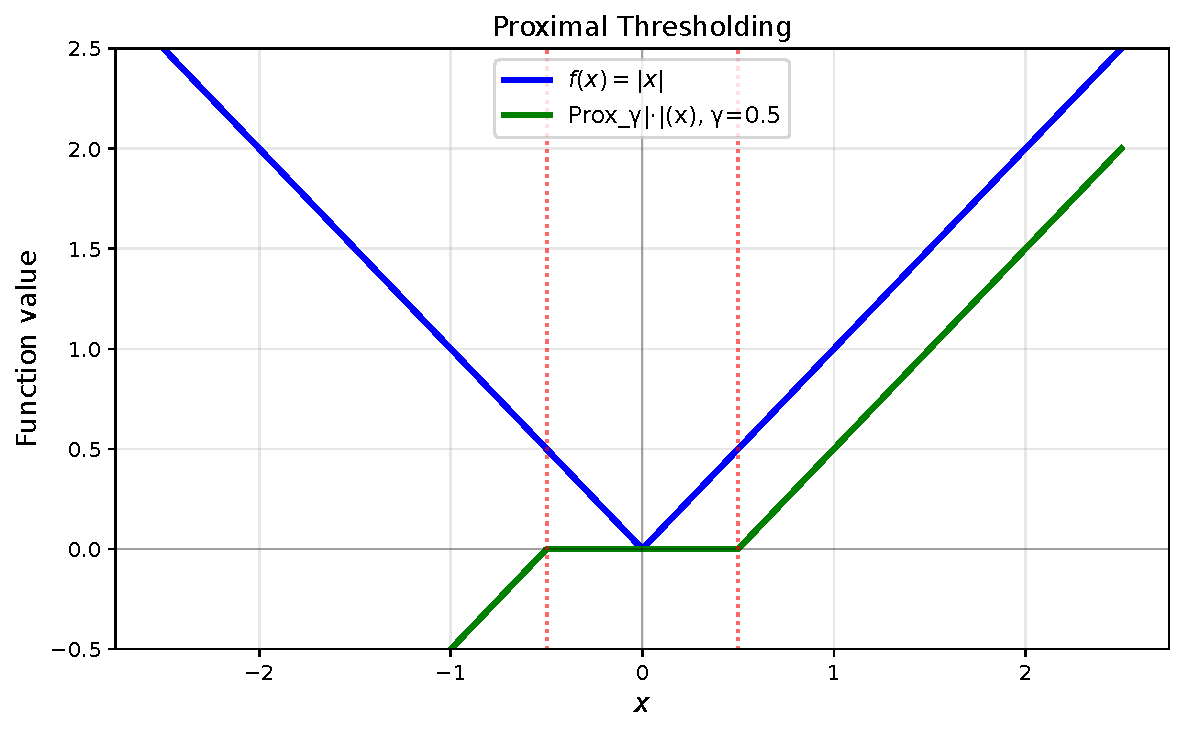
\includegraphics[width=0.5\textwidth]{fig_proximal_threshold.pdf}
\end{center}

\vspace{0.2cm}

Key applications:
\begin{itemize}
    \item Signal denoising (soft thresholding of wavelet coefficients)
    \item Sparse signal recovery
    \item $\ell_1$-regularized least squares problems
\end{itemize}
\end{frame}

\begin{frame}{Proximal Thresholding for Signal Processing}
\begin{example}[Soft Thresholding Signal Denoising]
Given a noisy signal $x \in \mathcal{H}$, the soft-thresholded version with threshold $\gamma$ is:
\[
\text{Prox}_{\gamma \|\cdot\|_1} x = \text{sign}(x) \max\{|x| - \gamma, 0\}
\]
\end{example}

\vspace{0.3cm}

\begin{itemize}
    \item Removes noise by thresholding coefficients
    \item Preserves signal energy better than hard thresholding
    \item Used extensively in wavelets and compressed sensing
\end{itemize}

\vspace{0.3cm}

\begin{exampleblock}{Application in $L^2$ Spaces}
For $\mathcal{H} = L^2(\Omega, \mathcal{F}, \mu)$ with measure $\mu$:
\[
P(\omega) = \text{soft}_{[-\gamma,\gamma]} X(\omega) = \text{sign}(X(\omega))\max\{|X(\omega)| - \gamma, 0\}
\]
Then $P = \mathrm{Prox}_{\gamma f} X$ where $f: \mathcal{H} \to \mathbb{R}$ is the appropriate convex function.
\end{exampleblock}
\end{frame}

%===============================================================================
\section{Numerical Examples and Algorithms}
%===============================================================================

\begin{frame}[fragile]{Proximal Gradient Descent Algorithm}

\begin{exampleblock}{Algorithm: Proximal Gradient Method}
Given $f, g \in \Gamma_0(\mathcal{H})$ and $x_0 \in \mathcal{H}$, set $\gamma \in (0, 2/L)$:
\begin{enumerate}
    \item Initialize: $x := x_0$, $t := 0$
    \item Repeat until convergence:
    \begin{enumerate}
        \item $x^{+} := \mathrm{Prox}_{\gamma f}(x - \gamma \nabla g(x))$
        \item $x := x^{+}$, $t := t + 1$
    \end{enumerate}
\end{enumerate}
\end{exampleblock}

\vspace{0.2cm}

\begin{lstlisting}
# Example: minimize ||Ax - b||^2/2 + gamma * ||x||_1
import numpy as np
from scipy.optimize import proximal_gradient_method

def soft_threshold(x, threshold):
    return np.sign(x) * np.maximum(np.abs(x) - threshold, 0)

def proximal_l1(x, gamma):
    return soft_threshold(x, gamma)

# Forward-backward splitting: minimize f(x) + g(x)
# where f is convex, g has L-Lipschitz gradient
\end{lstlisting}

\vspace{0.2cm}

\textbf{Convergence:} $x_t \to x^*$ as $t \to \infty$ under standard conditions.
\end{frame}

\begin{frame}[fragile]{Python Example: Soft Thresholding}

\begin{lstlisting}
import numpy as np
import matplotlib.pyplot as plt

def soft_threshold(x, gamma):
    """Soft thresholding operator (proximal of L1 norm)"""
    return np.sign(x) * np.maximum(np.abs(x) - gamma, 0)

# Example: Denoising
np.random.seed(42)
signal = np.array([1, 2, 3, 2, 1])
noise = np.random.normal(0, 0.5, len(signal))
noisy_signal = signal + noise

# Apply soft thresholding with gamma=0.5
gamma = 0.5
denoised = soft_threshold(noisy_signal, gamma)

print(f"Original:  {signal}")
print(f"Noisy:     {noisy_signal}")
print(f"Denoised:  {denoised}")

# Verify: check subdifferential condition
# For f(x) = gamma * ||x||_1:
# Prox_f(x) = soft_threshold(x, gamma)
\end{lstlisting}

\vspace{0.2cm}

Output illustrates how proximity operators remove noise while preserving structure.
\end{frame}

\begin{frame}{Convergence Analysis}
\begin{center}
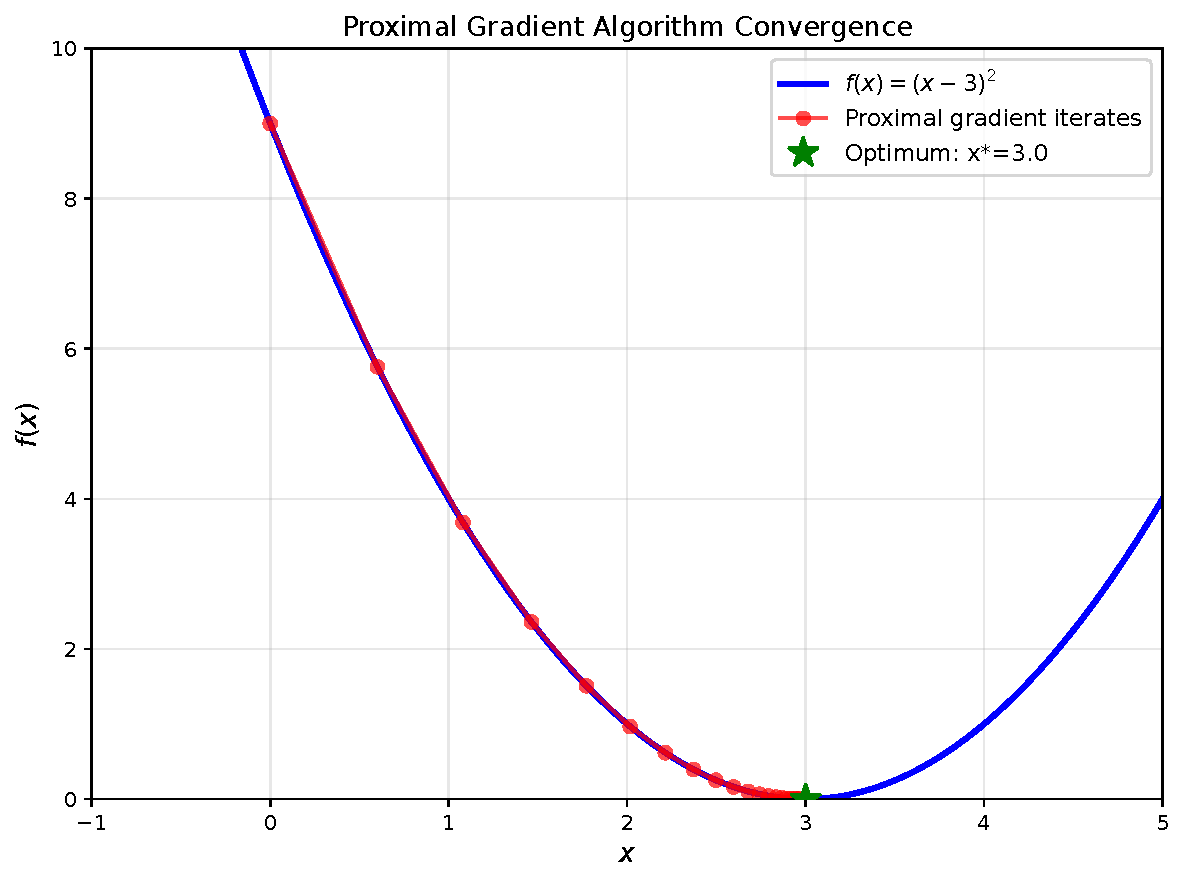
\includegraphics[width=0.7\textwidth]{fig_convergence.pdf}
\end{center}

\vspace{0.3cm}

\begin{theorem}[Convergence of Proximal Gradient Method]
Let $f, g \in \Gamma_0(\mathcal{H})$ with $g$ having $L$-Lipschitz continuous gradient. For $\gamma \in (0, 2/L)$, the iterates:
\[
x_{k+1} = \mathrm{Prox}_{\gamma f}(x_k - \gamma \nabla g(x_k))
\]
converge to a minimizer of $f + g$.
\end{theorem}
\end{frame}

%===============================================================================
\section{Perspective Functions}
%===============================================================================

\begin{frame}{Perspective Functions}
\begin{definition}[Perspective Function]
For $\varphi \in \Gamma_0(\mathcal{H})$ with $\mathrm{dom} \varphi^* = \mathcal{H}$, define:
\[
f: \mathbb{R} \times \mathcal{H} \to \mathbb{R} \cup \{+\infty\}, \quad (\xi, x) \mapsto \begin{cases}
\xi \varphi(x/\xi) & \text{if } \xi > 0 \\
(\mathrm{rec} \varphi)(x) & \text{if } \xi = 0 \\
+\infty & \text{if } \xi < 0
\end{cases}
\]
\end{definition}

\vspace{0.3cm}

\begin{theorem}[Proximity of Perspective Functions]
Let $(\xi, x) \in \mathbb{R} \times \mathcal{H}$ and $\gamma \in \mathbb{R}_{++}$. Then $f \in \Gamma_0(\mathbb{R} \oplus \mathcal{H})$ and:

If $\xi + \gamma\varphi^*(x/\gamma) \leq 0$: $\mathrm{Prox}_{\gamma f}(\xi, x) = (0, 0)$.
\end{theorem}

\vspace{0.3cm}

Applications in regularized optimization and hyperbolic constraints.
\end{frame}

%===============================================================================
\section{Advanced Topics}
%===============================================================================

\begin{frame}{Proximal Thresholders}
\begin{theorem}[Characterization of Proximal Thresholders]
Let $\Omega$ be a nonempty closed interval in $\mathbb{R}$ and $\phi \in \Gamma_0(\mathbb{R})$. Then the following are equivalent:
\begin{enumerate}
    \item $\mathrm{Prox}_\phi$ is a proximal thresholder on $\Omega$
    \item $\phi = \psi \oplus \sigma_\Omega$, where $\psi \in \Gamma_0(\mathbb{R})$ is differentiable at 0 with $\psi'(0) = 0$
\end{enumerate}
\end{theorem}

\vspace{0.3cm}

\begin{example}[Soft Threshold]
The soft thresholding operator (Example 24.20) is a proximal thresholder on $[-\gamma, \gamma]$.
\end{example}

\vspace{0.3cm}

Proximal thresholders provide a systematic way to understand and design operators for signal processing and optimization.
\end{frame}

\begin{frame}{Moreau Envelope}
\begin{definition}[Moreau Envelope]
The \textbf{Moreau envelope} of $f \in \Gamma_0(\mathcal{H})$ with parameter $\gamma > 0$ is:
\[
f^\gamma(x) := \inf_{p \in \mathcal{H}}\left(f(p) + \frac{1}{2\gamma}\|p - x\|^2\right)
\]
\end{definition}

\vspace{0.3cm}

\begin{properties}
\begin{enumerate}
    \item $f^\gamma$ is convex and continuously differentiable
    \item $\nabla f^\gamma(x) = \frac{1}{\gamma}(x - \mathrm{Prox}_{\gamma f}(x))$
    \item $f^\gamma(x) = \inf_p (f(p) + \frac{1}{2\gamma}\|p - x\|^2)$, with $p^* = \mathrm{Prox}_{\gamma f}(x)$
\end{enumerate}
\end{properties}

\vspace{0.3cm}

The Moreau envelope smooths $f$ and is fundamental to optimization algorithms.
\end{frame}

\begin{frame}{Properties of Moreau Envelope}
\begin{theorem}[Derivative of Moreau Envelope]
For $f \in \Gamma_0(\mathcal{H})$ and $\gamma \in \mathbb{R}_{++}$:
\[
(\forall x \in \mathcal{H})\quad \nabla f^\gamma(x) = \gamma^{-1}(x - \mathrm{Prox}_{\gamma f}(x))
\]
\end{theorem}

\vspace{0.3cm}

\begin{corollary}[Gradient Equivalence]
The proximity operator can be recovered from:
\[
\mathrm{Prox}_{\gamma f}(x) = x - \gamma \nabla f^\gamma(x)
\]
\end{corollary}

\vspace{0.3cm}

\begin{application}
The Moreau envelope is used in:
\begin{itemize}
    \item Smoothing nonsmooth functions for optimization
    \item Deriving algorithms with gradient-based structure
    \item Analyzing convergence rates
\end{itemize}
\end{application}
\end{frame}

%===============================================================================
\section{Applications in Optimization}
%===============================================================================

\begin{frame}{Lasso and Sparse Regression}
\begin{problem}[Lasso Problem]
Minimize:
\[
f(x) = \frac{1}{2}\|Ax - b\|_2^2 + \lambda\|x\|_1
\]
where $A \in \mathbb{R}^{m \times n}$, $b \in \mathbb{R}^m$, $\lambda > 0$.
\end{problem}

\vspace{0.3cm}

\begin{solution}[Proximal Gradient Method]
Iterate:
\[
x_{k+1} = \mathrm{Prox}_{\gamma \lambda \|\cdot\|_1}(x_k - \gamma A^T(Ax_k - b))
\]
where $\gamma \in (0, 2/\|A\|^2)$.
\end{solution}

\vspace{0.3cm}

The proximity operator of $\gamma\lambda\|\cdot\|_1$ is soft thresholding:
\[
\mathrm{Prox}_{\gamma\lambda\|\cdot\|_1}(z) = \text{sign}(z) \max\{|z| - \gamma\lambda, 0\}
\]
\end{frame}

\begin{frame}{Matrix Completion and Nuclear Norm Minimization}
\begin{problem}[Matrix Completion]
Minimize:
\[
f(M) = \frac{1}{2}\|P_\Omega(M - M^*)\|_F^2 + \lambda \|M\|_*
\]
where $\|M\|_*$ is the nuclear norm (sum of singular values).
\end{problem}

\vspace{0.3cm}

\begin{solution}[Proximal Operator of Nuclear Norm]
For $M \in \mathbb{R}^{m \times n}$ with SVD $M = U\Sigma V^T$:
\[
\mathrm{Prox}_{\gamma \|\cdot\|_*}(M) = U \Sigma_\gamma V^T
\]
where $\Sigma_\gamma = \mathrm{Diag}(\mathrm{Prox}_\gamma(\sigma_1), \ldots, \mathrm{Prox}_\gamma(\sigma_r), 0, \ldots, 0)$.
\end{solution}

\vspace{0.2cm}

This reduces to soft thresholding of singular values.
\end{frame}

\begin{frame}[fragile]{Proximal Splitting Algorithms}

\begin{exampleblock}{Algorithm: Douglas-Rachford Splitting}
To minimize $f(x) + g(x)$ where $f, g \in \Gamma_0(\mathcal{H})$:
\begin{enumerate}
    \item Initialize: $y_0 \in \mathcal{H}$
    \item Repeat: $x_{k+1} = \mathrm{Prox}_f(y_k)$, \quad $y_{k+1} = y_k + \mathrm{Prox}_g(2x_{k+1} - y_k) - x_{k+1}$
\end{enumerate}
Converges to a minimizer of $f + g$ under standard conditions.
\end{exampleblock}

\vspace{0.3cm}

\begin{lstlisting}
# Douglas-Rachford splitting
def douglas_rachford(f_prox, g_prox, y0, max_iter=100):
    y = y0
    for k in range(max_iter):
        x = f_prox(y)           # Prox_f
        g_eval = g_prox(2*x - y)  # Prox_g
        y = y + g_eval - x
    return x
\end{lstlisting}

\vspace{0.2cm}

Key advantage: Handles cases where minimizing $f + g$ directly is difficult.
\end{frame}

%===============================================================================
\section{Functions on Matrices}
%===============================================================================

\begin{frame}{Proximity Operators on Matrix Spaces}
\begin{theorem}[Singular Value Thresholding]
Let $\phi \in \Gamma_0(\mathbb{R})$ be even and $A \in \mathbb{R}^{M \times N}$ with SVD $A = U\Sigma V^T$. Then:
\[
\mathrm{Prox}_\phi(A) = U\Sigma_\phi V^T
\]
where $\Sigma_\phi = \mathrm{Diag}(\mathrm{Prox}_\phi(\sigma_1), \ldots, \mathrm{Prox}_\phi(\sigma_r), 0, \ldots, 0)$.
\end{theorem}

\vspace{0.3cm}

\begin{example}[Nuclear Norm Proximity]
For the nuclear norm $\|A\|_* = \sum_i \sigma_i$:
\[
\mathrm{Prox}_{\gamma\|\cdot\|_*}(A) = U\Sigma_\gamma V^T
\]
where $\Sigma_\gamma = \mathrm{Diag}(\max\{\sigma_1 - \gamma, 0\}, \ldots)$ (soft threshold on singular values).
\end{example}

\vspace{0.3cm}

Applications:
\begin{itemize}
    \item Matrix completion
    \item Low-rank approximation
    \item Robust PCA
\end{itemize}
\end{frame}

%===============================================================================
\section{Summary and Key Takeaways}
%===============================================================================

\begin{frame}{Summary: Core Concepts}
\begin{itemize}
    \item \textbf{Proximity Operator:} Balances minimizing a convex function $f$ with staying close to a point $x$

    \vspace{0.2cm}

    \item \textbf{Characterization:} $p = \mathrm{Prox}_{\gamma f}(x) \iff x - p \in \gamma \partial f(p)$

    \vspace{0.2cm}

    \item \textbf{Key Property:} Single-valued, nonexpansive operator with strong convergence properties

    \vspace{0.2cm}

    \item \textbf{Special Cases:}
    \begin{enumerate}
        \item Projections onto convex sets
        \item Soft thresholding (for $\ell_1$ norm)
        \item Singular value thresholding (for nuclear norm)
    \end{enumerate}

    \vspace{0.2cm}

    \item \textbf{Moreau Envelope:} $f^\gamma(x) = \inf_p(f(p) + \frac{1}{2\gamma}\|p-x\|^2)$ provides smoothing

    \vspace{0.2cm}

    \item \textbf{Algorithms:} Proximal gradient method, Douglas-Rachford splitting, ADMM
\end{itemize}
\end{frame}

\begin{frame}{Key Results}
\begin{enumerate}
    \item Proximity operators are resolvent operators of the subdifferential
    \vspace{0.15cm}

    \item They inherit important properties:
    \begin{itemize}
        \item Weak sequential continuity
        \item Nonexpansiveness: $\|\mathrm{Prox}_f x - \mathrm{Prox}_f y\| \leq \|x - y\|$
        \item Fixed points correspond to minimizers of $f$
    \end{itemize}

    \vspace{0.2cm}

    \item Composition rules enable flexible operator design

    \vspace{0.15cm}

    \item Explicit formulas available for:
    \begin{itemize}
        \item Quadratic functions
        \item Norms ($\ell_1$, nuclear norm, etc.)
        \item Indicators of convex sets
        \item Distance functions
    \end{itemize}

    \vspace{0.2cm}

    \item Moreau envelope: Key tool for smoothing and algorithm design

    \vspace{0.15cm}

    \item Proximal algorithms (FISTA, ADMM, etc.) are among the most efficient modern methods
\end{enumerate}
\end{frame}

\begin{frame}{Applications Across Domains}
\begin{block}{Signal Processing}
\begin{itemize}
    \item Denoising via soft thresholding
    \item Compressed sensing
    \item Wavelet shrinkage
\end{itemize}
\end{block}

\begin{block}{Optimization and Machine Learning}
\begin{itemize}
    \item Lasso and sparse regression
    \item Matrix completion
    \item Robust PCA
    \item Convex optimization algorithms
\end{itemize}
\end{block}

\begin{block}{Statistical Learning}
\begin{itemize}
    \item Regularized regression
    \item Feature selection
    \item Smoothing in high dimensions
\end{itemize}
\end{block}
\end{frame}

\begin{frame}[allowframebreaks]{Further Reading}
Key references from Chapter 24:
\begin{itemize}
    \item Proposition 24.1-24.30: Core theory of proximity operators
    \item Theorem 24.52: Proximal thresholders characterization
    \item Examples 24.1-24.66: Extensive worked examples
    \item Sections 24.4-24.8: Applications and special cases
\end{itemize}

\vspace{0.3cm}

For practical algorithm implementations:
\begin{itemize}
    \item Proximal gradient method (forward-backward splitting)
    \item Douglas-Rachford splitting
    \item ADMM (Alternating Direction Method of Multipliers)
    \item FISTA (Fast Iterative Shrinkage-Thresholding Algorithm)
\end{itemize}

\vspace{0.3cm}

Modern optimization frameworks:
\begin{itemize}
    \item ProximalAlgorithms.jl (Julia)
    \item CVX (MATLAB)
    \item Scikit-optimize (Python)
\end{itemize}
\end{frame}

\end{document}
